%=====================================================
%
% Variables (same scheme as the sample document)
%
%=====================================================

\def\doctype{article}

\def\emptypages{false}
\def\showparts{false}

\def\ttitlepage{titlepage.tex}
\def\ttitlepagetitletop{Engines, Quantisation, and the Harness}
\def\ttitlepagesubtitletop{Inkling 2 Mini, Hy4-Flash, and Signal 2 as Local Coding Workers}
\def\ttitlepagetitlemiddle{Lab Report}
\def\ttitlepagesubtitlemiddle{Measurements of 21--23 November 2026}

\def\torganization{Independent Research}
\def\tsubmissiondate{23 November 2026}
\def\tversion{0.1 (draft)}
\def\tauthor{Matthias Nott}
\def\tcontact{~}
\def\tcontactid{~}

\def\tfooterleftlabelup{Title}
\def\tfooterleftlabeldown{Author}
\def\tfooterleftup{Local Coding Agents, Report 5}
\def\tfooterleftdown{Matthias Nott}
\def\tfootermiddleup{Engines and Harness}
\def\tfootermiddledown{Lab Report}
\def\tfooterrightlabelup{Date}
\def\tfooterrightlabeldown{Version}
\def\tfooterrightup{November 2026}
\def\tfooterrightdown{0.1}

\def\showtitlepage{true}
\def\showlistofs{true}
\def\showtoc{true}
\def\showlot{true}
\def\showlof{false}
\def\showloe{false}
\def\showlod{false}

\def\showreferences{true}
\def\showappendix{false}
\def\showendnotes{false}
\def\showanyglossary{false}
\def\showacronyms{false}
\def\showglossary{false}
\def\showstatic{false}
\def\showindex{false}

\def\showpageheaders{true}
\def\showpagefooters{true}
\def\showwordcount{false}
\def\showwordcountback{false}

\input{templates/cfg/zz_layout}

\setcounter{tocdepth}{2}

\usepackage[
  style=apa
, citestyle=authoryear
, backend=biber
, maxnames=3
, minnames=1
, sorting=nyt
, sortcites=true
, block=space
, safeinputenc
, natbib=true
, backref=true
, uniquename=init]{biblatex}
\DeclareLanguageMapping{american}{american-apa}
\addbibresource{Bibliography.bib}
\input{templates/cfg/zz_config_bib}

\usepackage{indentfirst}

\newcommand{\cmd}[1]{\texttt{#1}}

% Alternate row colours in every table (xcolor is loaded with the table option by the layout)
% Breathing room between tables and the running text
\setlength{\intextsep}{16pt plus 2pt minus 2pt}
\setlength{\textfloatsep}{18pt plus 2pt minus 4pt}
\setlength{\floatsep}{16pt plus 2pt minus 2pt}

\definecolor{rowtint}{gray}{0.93}
\AtBeginEnvironment{table}{\global\csname @rowcolorstrue\endcsname\rowcolors{2}{rowtint}{white}}
\newcolumntype{P}[1]{>{\raggedright\arraybackslash}p{#1}}
\setcounter{secnumdepth}{2}
\newcommand{\todo}[1]{\textcolor{red}{[TODO: #1]}}

\begin{document}

%=====================================================
% Title page and abstract
%=====================================================

\input{tex/\ttitlepage}

\begin{center}
\begin{minipage}{0.86\textwidth}
\section*{Abstract}

The fourth report fixed the roles of a local worker and a cloud planner. This fifth report asks which local model and
which serving engine should fill the worker role, and what the agent harness contributes. On one workstation with
128\,GB of unified memory, ten setups were run through the same bench: 20 questions, 40 easy and 40 hard function
tasks written to disk without execution, and five repository changes graded by hidden tests. Gyro-L on Strata is the
reference (19/20, 38/40, 35/40, 10 of 10 real tasks over two clean runs). Signal 2, a smaller model on the same engine,
reaches the function-level sets within three tasks and passes 8 of 10 real tasks with about 31\,GB on the GPU against 76\,GB wired for Gyro-L; two instances
side by side pass 8 of 10 as well and deliver 6.85 passed real tasks per hour against 4.56 for one Gyro-L. Inkling 2 Mini
is fast and passes the function sets, but passes 2--3 of 5 real tasks on every MLX engine and on Strata. Of its 22
real-task failures 12 are stalls (no edit in 20 minutes) and 7 are faults of our harness; only 2 are loops and 1 is a wrong
fix. Fixing the harness faults and rewriting the stall and loop rules changed behaviour (edits from minute 6 instead of a 20-minute stall) and gave 3 of 4 tasks on one validation run; the loop guard turned out to be blind because other hooks rewrite tool input. Three Strata
releases changed no kernel that Gyro-L uses; a barrier-free GEMV patch is bit-identical and unmeasurable. All
real-task results rest on one or two runs of five self-written tasks on one machine.

\end{minipage}
\end{center}

\clearpage

%=====================================================
% Table of contents and list of tables
%=====================================================

\sequals{\showpageheaders}{true}{
	\pagestyle{fancy}
	\fancyhead{}
	\fancyhead[RO,LE]{\thepage}
	\fancyhead[LO]{\slshape CONTENTS}
	\fancyhead[RE]{\slshape CONTENTS}
}{}
\sequals{\showpagefooters}{true}{\fancyfoot[C]{}}{}
\pdfbookmark[-1]{\contentsname}{toc}
\tableofcontents
\addtocontents{lot}{\protect\vspace{10pt}}
\listoftables
\clearpage

\sequals{\showpageheaders}{true}{
	\pagestyle{fancy}
	\fancyhead{}
	\fancyhead[LE,RO]{\thepage}
	\fancyhead[RE]{\slshape \rightmark}
	\fancyhead[LO]{\slshape \rightmark}
}{}
\sequals{\showpagefooters}{true}{\fancyfoot[C]{\pfooter}}{}
\renewcommand{\sectionmark}[1]{\markboth{\thesection.\ #1}{\thesection.\ #1}}
\renewcommand{\subsectionmark}[1]{}
\clearpage

%=====================================================
% Body
%=====================================================

\section{Introduction}\label{sec:intro}

Report 4 treated the local worker as given and asked how to use it. The worker itself was one model, Gyro-L, on one
engine, Strata \citep{Strata-2026aa}. In the three days of this report the field around it moved: a new family of
models (Inkling 2 Mini) became runnable on four engines, a second Strata family (Hy4-Flash) appeared, a smaller
fine-tune of the Gyro family (Signal 2) was released, and Strata itself shipped three versions. The questions are
which of these is a better worker than the reference, whether the engine matters as much as the model, and how much
of what looks like a model weakness is a fault of the harness around it. All workers were started through PAI
\citep{Nott-2026aa} with Claude Code as the agent harness \citep{Anthropic-2026aa}; the harness adds loop guards, path
repair and a router that translates between the agent's API and the local server.

\section{Setting}\label{sec:setting}

\subsection{Machine, engines and models}

One Apple M5 Max with 128\,GB unified memory; one GPU job at a time, with one exception described in
Section~\ref{sec:dual}. Strata is a Metal engine with its own kernels; Locals \citep{Locals-2026aa} and MTPLX
\citep{MTPLX-2026aa} are servers on top of MLX \citep{MLX-2026aa}; oMLX was used only in earlier direct tests.

\begin{table}[H]
\centering
\small
\caption{Setups of this report}\label{tab:setups}
\begin{tabular}{P{3.7cm}P{2.9cm}P{7.0cm}}
\toprule
Setup & Engine & Note \\
\midrule
Gyro-L & Strata 0.2.18 & Reference worker of report 4; 76\,GB wired \\
Signal 2 & Strata 0.2.18 & Smaller Gyro fine-tune, about 31\,GB on the GPU; one or two instances \\
Inkling, Locals & Locals & 4-bit float weights plus draft model, 15.55\,GB on disk \\
Inkling, MTPLX & MTPLX 2.13.1/2.13.2 & Four reasoning efforts: default 0.9, medium 0.7, low 0.2, off \\
Inkling, Strata & Strata 0.2.19 & Thinking switched off only \\
Hy4-Flash & Strata 0.2.18 & Direct tests and two worker tasks, not in the bench \\
\bottomrule
\end{tabular}
\end{table}

\subsection{Bench}

\emph{short}: 20 questions with exact answers. \emph{easy} and \emph{hard}: 40 function-level Python tasks each; the
worker may only read and write files, so nothing can be executed and the answer is what it writes; graded by hidden
tests. \emph{real}: five changes from the PAI repository (prune-dist-rerun, mirror-sync-token, worker-priority,
session-move-selectors, escalate-loopstop) graded by hidden behaviour tests, each with a 30-minute deadline and a
20-minute allowance without progress. The task prune-dist-rerun is confounded by the machine: its visible test is
red before any edit because it reads the live process list and the process start time is printed in the system
locale. Gyro-L passed it only because its early edit was right and the run was stopped at the deadline. It is kept in the
counts and called out where it matters. Each cell below is one run unless stated.

\section{Results}\label{sec:results}

\subsection{Pass rate and time per setup}

Table~\ref{tab:sets} and Figure~\ref{fig:pass} give the four sets. Gyro-L is the only setup that passes everything
real; on the function sets the differences between the best setups are two to four tasks of 40, which is within
what one run cannot resolve.

\begin{table}[H]
\centering
\small
\caption{Passed tasks and wall time per set (one run each; Gyro-L real and Signal 2 real: see text for further runs)}\label{tab:sets}
\resizebox{\textwidth}{!}{\begin{tabular}{lrrrr}
\toprule
Setup & short (20) & easy (40) & hard (40) & real (5) \\
\midrule
Gyro-L & 19, 54\,s & 38, 6.7\,min & 35, 8.8\,min & 5, 65\,min \\
Signal 2, solo & 16, 52\,s & 38, 5.5\,min & 33, 9.0\,min & 5, 67\,min \\
Signal 2, dual A (parallel) & 17, 70\,s & 38, 6.5\,min & 31, 14\,min$^{a}$ & 4, 67\,min \\
Signal 2, dual B (parallel) & 17, 74\,s & 37, 13\,min & 34, 19\,min & 4, 74\,min \\
Inkling, Locals & 18, 69\,s & 39, 5.9\,min & 36, 12.5\,min & 3, 25\,min \\
Inkling, MTPLX default (0.9) & 20, 4.8\,min & 39, 10.6\,min & 37, 38\,min & 2, 93\,min$^{b}$ \\
Inkling, MTPLX low (0.2) & 20, 2.5\,min & 40, 2.8\,min & 36, 10\,min & 3, 30\,min$^{c}$ \\
Inkling, MTPLX medium (0.7) & 18, 1.6\,min & 40, 7.6\,min & 33, 37\,min & 3, 81\,min \\
Inkling, MTPLX off & 19, 2.0\,min & 40, 9.5\,min & 36, 56\,min & 2, 76\,min \\
Inkling, Strata 0.2.19 & 17, 68\,s & 3, 75\,s$^{d}$ & 7, 14\,min$^{d}$ & 2, 72\,min \\
\bottomrule
\end{tabular}}
\par\smallskip{\footnotesize\raggedright $^{a}$ The first hard run of instance A failed in 19\,s (instrument fault, 0/40) and is discarded; the repeat is shown. $^{b}$ Repeat after a router fault had cost the first run (0/5). $^{c}$ Two runs, 3/5 each. $^{d}$ The model loops on an unavailable shell command; the first two attempts (0/40) were a router fault, see Section~\ref{sec:harness}. Gyro-L and Signal~2 solo have further real-task runs: Gyro-L 5/5 (66\,min), Signal~2 3/5 (55\,min). A second Gyro-L real run was lost to a machine crash and is not counted.\par}
\end{table}

\begin{figure}[H]
\centering
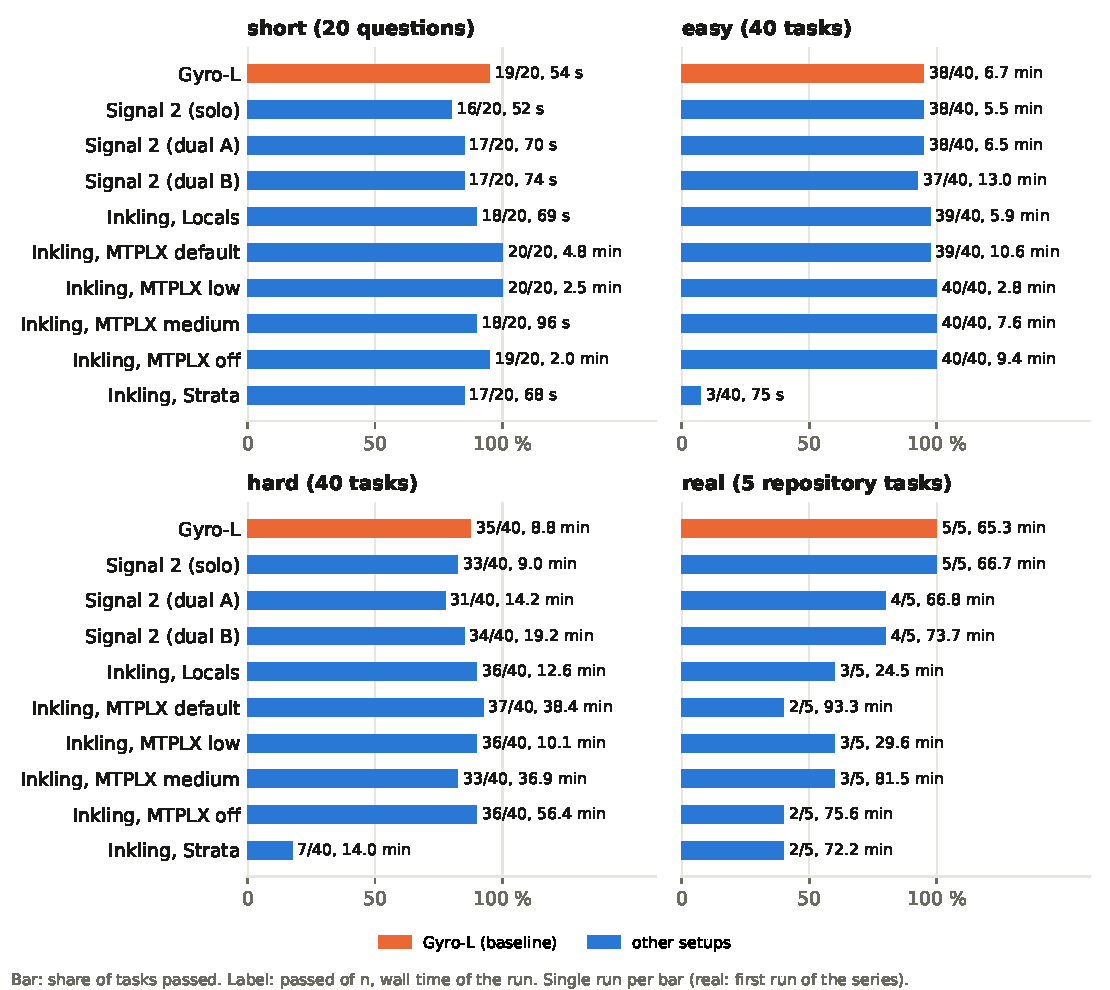
\includegraphics[width=\textwidth]{figures/fig-pass-rate.pdf}
\caption{Pass rate per set and setup. Orange is the Gyro-L baseline. Labels give passed tasks and wall time.}\label{fig:pass}
\end{figure}

On the five real tasks the Inkling variants finish 2--3 and are faster per task when they pass: a pass costs
them 1 to 8 minutes (mirror-sync-token 64--137\,s, session-move-selectors 107--195\,s, escalate-loopstop
126--716\,s) against 5--14 minutes for Gyro-L. Their failures cost 20 minutes each, the length of the no-progress
allowance, which is why the whole-run time of several variants is longer than Gyro-L's
(Figure~\ref{fig:real}). The reasoning effort does not buy quality: low (0.2) is as good as the others on every
set and several times faster than default (0.9), medium and off on the hard set (10 against 38, 37 and 56 minutes).
Across the hard set the failures of Inkling low (four) and Signal 2 (seven) are wrong answers, with no overlap
between the two models' failed tasks; in this set no hook can help, because nothing can be executed.

\begin{figure}[H]
\centering
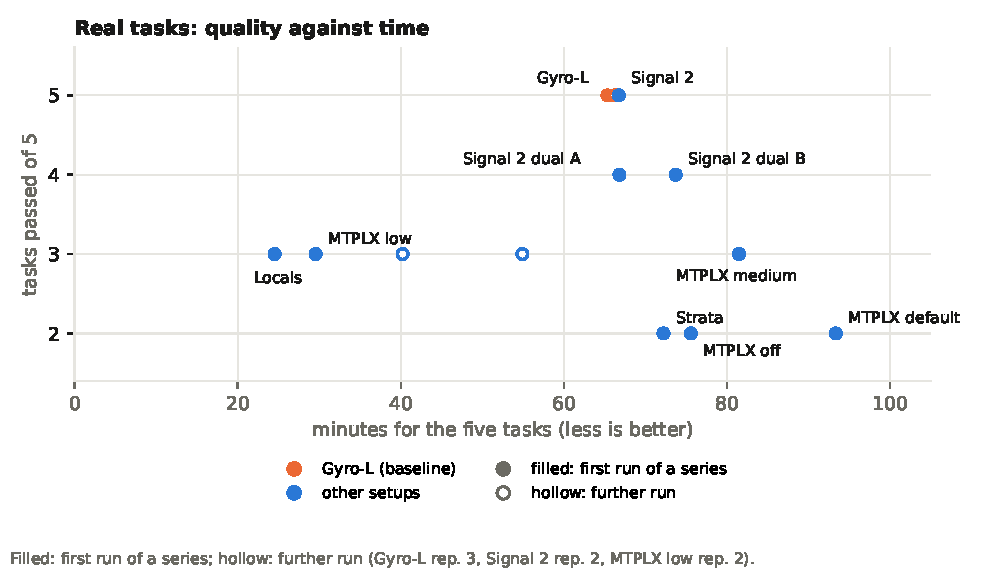
\includegraphics[width=0.85\textwidth]{figures/fig-real-quality-time.pdf}
\caption{Real tasks: passed against minutes for the five tasks. Filled marks are the first run of a series.}\label{fig:real}
\end{figure}

\subsection{Two Signal 2 instances}\label{sec:dual}

Signal 2 needs about 31\,GB on the GPU, so two instances (2 $\times$ about 41\,GB resident, 58.5\,GB wired in total;
Gyro-L alone wires 76\,GB) fit next to each other. The full bench was run on both at once, with its own
conversation cache for each. Table~\ref{tab:dual} compares them with the single servers on the real tasks.

\begin{table}[H]
\centering
\small
\caption{Real tasks, Gyro-L and Signal 2 on one server and two instances in parallel}\label{tab:dual}
\begin{tabular}{lrrrr}
\toprule
Setup & Runs & Passed & Seconds per run & Passed per hour \\
\midrule
Gyro-L, one server & 2 & 10/10 & 3920, 3975 & 4.56 \\
Signal 2, one server & 2 & 8/10 & 4003, 3294 & 3.95 \\
Signal 2, instance A of two & 1 & 4/5 & 4008 & 3.59 \\
Signal 2, instance B of two & 1 & 4/5 & 4422 & 3.26 \\
Signal 2, A and B together & & 8/10 & & 6.85 \\
\bottomrule
\end{tabular}
\par\smallskip{\footnotesize\raggedright Passed per hour is passed tasks over the summed run time. The combined figure adds the rates of A and B, each measured while the other instance was busy (for 81 minutes both ran without a break). The 30-minute deadline of prune-dist-rerun is part of every run.\par}
\end{table}

\begin{figure}[H]
\centering
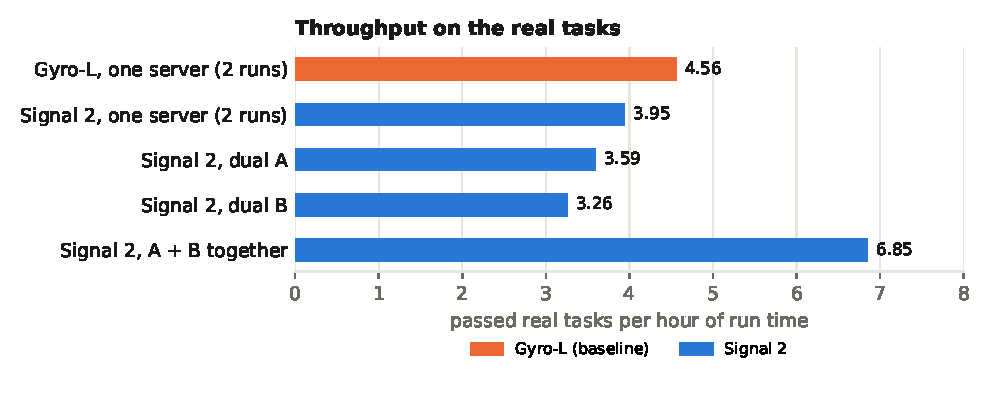
\includegraphics[width=0.85\textwidth]{figures/fig-throughput.pdf}
\caption{Passed real tasks per hour of run time.}\label{fig:thr}
\end{figure}

Running two instances kept quality (8 of 10, as for one instance over its two runs) and cost each instance
about 10 to 21 percent more run time (4008 and 4422\,s against the single-instance mean of 3649\,s, the mean of 4003 and 3294\,s). With passed per hour = passed tasks $/$ run time $\times$ 3600\,s, one instance gives 3.95 (4 passes in 3649\,s), the two instances 3.59 + 3.26 = 6.85, so throughput rose by 6.85\,$/$\,3.95 = 1.7 times, not 2 times; against Gyro-L (4.56) it is 1.5 times. The whole-run output speed of each instance fell to 8.9 and 11.4 tokens/s
from 18.6, but those figures include waiting. Both instances failed prune-dist-rerun, the confounded task. On the
function sets the dual runs match the single run within one to two tasks (short 17 and 17 against 16, easy 38 and 37
against 38, hard 31 and 34 against 33); instance B needed 13 minutes for the easy set where one instance needed 5.5.
The dual bench ran for 106 minutes without a fault.

A token comparison with Gyro-L could not be made from the raw files: the loop-stopped Gyro-L runs and its
deadline-killed task carry no token count. An earlier note quoted 25--30\,\% fewer output tokens for Signal 2; the
raw real-task files show more (74 thousand against 29 thousand), so that figure is not used here.

\subsection{Hy4-Flash}

Hy4-Flash (Strata 0.2.18, SQ-64 pack) was tested directly and with two worker tasks, not in the bench. Direct tests
passed 6 of 6 small coding tasks; for tool calls the reasoning effort must be \emph{high}, in \emph{no think} the
tool call is answered in prose. As shipped it re-read the whole prompt on every worker turn (25 thousand tokens, about
100\,s per turn) because the engine reused a prompt only when the whole previous sequence was its prefix. After
adding prefix reuse, conversation slots and a disk tier to the engine, a repeated 46-thousand-token prompt dropped from
44\,s to 0.3\,s and an agent-style turn of 17 thousand tokens from 20--22\,s to 1.1--1.3\,s. Result: the budget task
passed twice (4/5 on review each time, 15--16 minutes against 5.7 for Gyro-L), the test-hint task failed three
times with the same mistake (its own new test expected a denial that the fixture never triggers), once even with the
maximum reasoning effort, where it named the cause correctly and still stopped. Hy4-Flash is a usable worker, not a
better one; it is not in any routing chain.

\section{Failure analysis}\label{sec:failures}

\subsection{Taxonomy}

The 22 non-passes of the real set over the eight Inkling runs were classified from the replayed transcripts:
A loop, B stall (no edit), C wrong fix, D gave up, E fault of our harness (Figure~\ref{fig:fail}). Counts:
\textbf{B 12, E 7, A 2, C 1, D 0}. The dominant failure is exploring, not looping: in 11 of the 12 stalls the model made no
single edit in 20 minutes, with 50 to 94 read-only calls, until the no-progress allowance stopped it. Gyro-L made its
first edit after 7 and 9 calls (1.3 and 3.4 minutes) on the two tasks compared and used the edit tool 22 to 45 times; Inkling used it
in none of its failed runs. The specification of every stalled task names the two to four files to open; the model
read them in the first minute and then kept looking for where a setting comes from.

\begin{figure}[H]
\centering
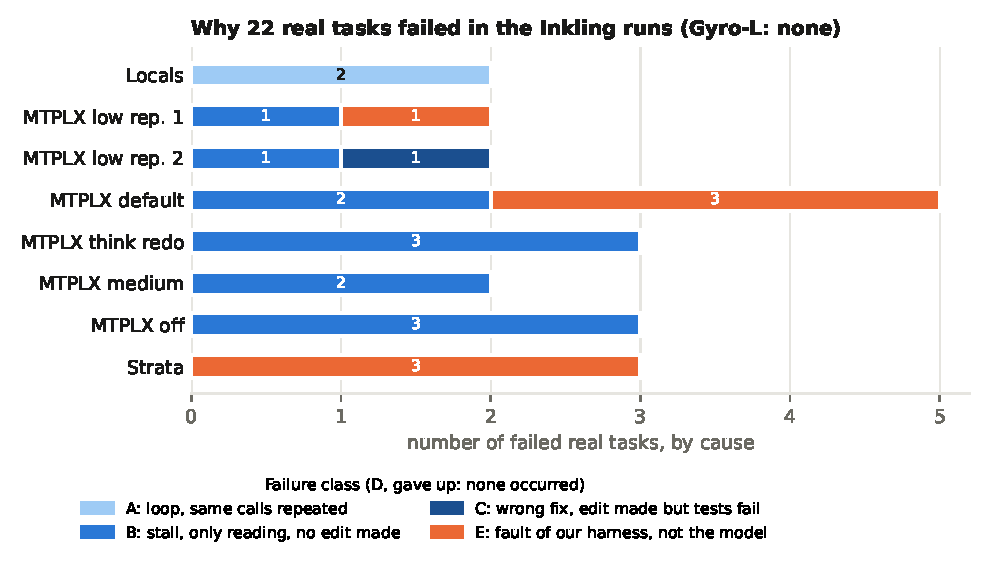
\includegraphics[width=0.85\textwidth]{figures/fig-failure-classes.pdf}
\caption{Classes of the 22 failed real tasks of the Inkling runs, one bar per run. Colours: A, loop (light blue); B, stall, only reading and no edit (blue); C, wrong fix, an edit that fails the tests (dark blue); E, fault of our harness (orange); D, gave up, did not occur. Gyro-L had none in its clean runs.}\label{fig:fail}
\end{figure}

Two faults of the existing guards made the stalls longer. The note of the loop guard fired from the first minute and
kept firing (8 to 22 times per stalled run) with no effect, because it said ``if your change is complete and its
checks passed, stop checking'' to a model that had changed nothing. A redirect text existed, but it was keyed to one exact
model identifier and the engines report other identifiers, so it was inactive in 20 of the 22 failures.

\subsection{Harness faults found and fixed}\label{sec:harness}

Seven failures and several zero-score runs were faults of our own harness. All were fixed and merged during the
three days:

\begin{itemize}
\item \textbf{Router, held replies.} A reply held back by the tool-name fixer was re-sent without its completion
flag, so every held answer was logged as ``closed mid-answer'' (13,419 lines for Gyro-L) and large answers were cut
without a stop message. After the fix: 0 such lines against 408 Gyro-L answers.
\item \textbf{Router, tool-call assembly.} MTPLX sent parallel tool calls with concatenated arguments
\citep{MTPLX-2026ab}; the router now splits them. MTPLX 2.13.2 fixes it at the source (verified 3 of 3). The first
MTPLX real run scored 0/5 for this reason.
\item \textbf{Text tool calls for undeclared tools.} A model that writes a tool call as text for a tool the request does not
declare was not parsed; for every local provider the call is now passed on. The first Strata sets scored 0/0/0 for this
reason; afterwards the model looped on an unavailable shell command.
\item \textbf{Output limits.} Three tasks of one run ended after 5\,s with ``cut off before its arguments were complete'';
runaway single turns of more than 32 thousand tokens killed three Strata runs; an output cap of 12,000 tokens for Inkling
was added. Loop-stopped runs now keep their token usage.
\item \textbf{Loop guard blind to results.} The guard compared commands and results to detect repetition, but other hooks
(a command-prefixing hook, the read-path repair) rewrite the tool input after the guard has seen it, so most results could not be
matched (null for most calls). Different windows of the same file were counted as the same command and denied. The guard
was fixed to see the results of rewritten calls, and null results are no longer counted as equal.
\item \textbf{Guard false positive.} A compound command holding the real fix followed by a test run was denied as a whole
because of its test tail; the worker, with a correct fix, was stopped. Writes inside compound commands are allowed now, and
identical red test runs are no longer counted as progress.
\item \textbf{Sleep and server guards, merge targets, JSON output.} Sleep limits apply per step; a worker's merge goes to
the linked worktree it started in; JSON output of CLI commands is kept clean on stdout; a leaked test process had run at 98\,\% CPU for
23 hours across all bench runs and is now reaped.
\end{itemize}

\subsection{New rules and their validation}

From the taxonomy came: a no-edit stall rule (a note after 12 calls or 4 minutes without an edit, a second after 25 and 8,
reads denied after 40 and 12), per-model texts matched by pattern instead of exact identifier, content fingerprints for repeated
failures, an extended baseline-red text and the output cap. Validation was a re-run of four real tasks (prune-dist
included, mirror-sync-token excluded): MTPLX 2.13.1 low with the rules passed 2 of 4; on worker-priority the model now
edited from minute 6 instead of stalling for 20 minutes, but the fix was wrong. MTPLX 2.13.2 low with the rules passed
3 of 4, including prune-dist-rerun for the first time (7.3 minutes); worker-priority still failed. Worker-priority fails on every
Inkling engine; only Gyro-L and Signal 2 pass it. A Locals re-run with the older redirect note (two tasks) passed
one; the note never fired. These are single runs of four tasks; the rules are shown to move behaviour, not to lift the pass
rate with any confidence.

\section{Engine notes}\label{sec:engines}

\begin{figure}[H]
\centering
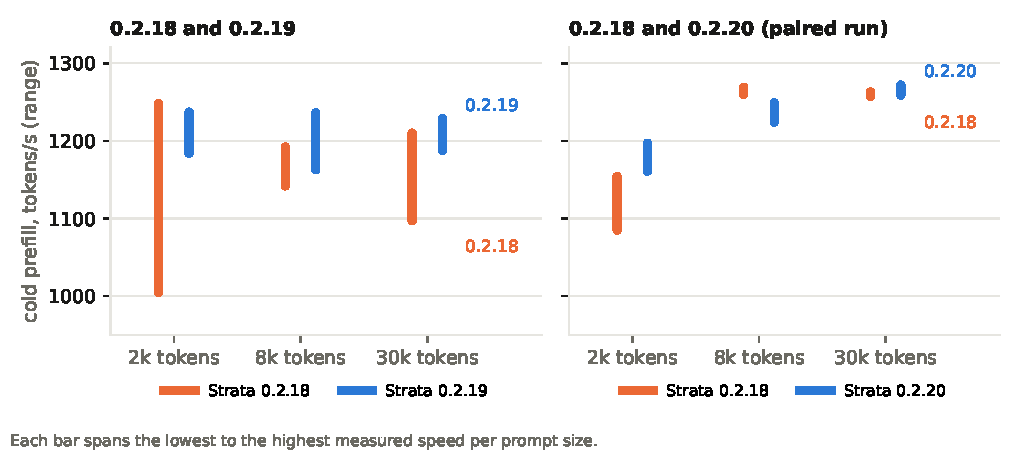
\includegraphics[width=0.95\textwidth]{figures/fig-prefill-versions.pdf}
\caption{Gyro-L cold prefill speed by Strata version, ranges over the measured prompts (2, 8 and 30 thousand tokens); orange is 0.2.18, blue the newer version named in the legend.
Left: earlier A/B; right: paired run with identical prompts. Decode: 74--78 tokens/s on 0.2.18 and 0.2.19, 75--80 on 0.2.20.}\label{fig:prefill}
\end{figure}

\paragraph{Strata 0.2.19 and 0.2.20.} The diff of 0.2.19 is 278 files and 81.6 thousand lines, but the Metal engine
changed in three files and in no kernel; of everything that is compiled for Gyro-L exactly one change can alter speed
(a threaded decode of the per-layer embedding rows, prefill only, bit-identical by construction). The release notes' +40\,\%
for the Flash-Next family concerns NVIDIA and AMD kernels. Measured (Figure~\ref{fig:prefill}): prefill 1005--1248 tokens/s
on 0.2.18 against 1163--1237 on 0.2.19, ranges overlapping, decode equal. 0.2.20 produced the same output hashes on all six prompts
as 0.2.18 and the same speed. All three Strata servers stay on one of these builds without a reason to choose.
Our three earlier Strata pull requests, the persistent SSD tier and the Hy4-Flash session reuse and memory fixes (\href{https://github.com/Niko1221/Strata/pull/6538}{\#6538}, \href{https://github.com/Niko1221/Strata/pull/6539}{\#6539}, \href{https://github.com/Niko1221/Strata/pull/6540}{\#6540}), were integrated into 0.2.20 by the maintainers; findings are collected in issue \href{https://github.com/Niko1221/Strata/issues/6542}{\#6542}.

\paragraph{GEMV barrier skip.} A decode kernel variant that skips a load and a barrier for formats without a lookup
table gave bit-identical output on 12 of 12 prompts and decode of 61--74 against 61--73 tokens/s on identical prompts: no
measurable gain, not proposed upstream.

\paragraph{MLX attention fix.} MLX fixed a register spill in its decode attention for keys with more than 512 value
dimensions. Strata has no global tile constant; a static read of each decode kernel gives 35--70 live registers per
thread for the Gyro-L and Inkling kernels, about 55 for the Hy4 non-MPP kernel, and a borderline 90--115 for two
Hy4 kernels (one of them not dispatched). These are hand estimates from the source, not compiler output.

\paragraph{Disk tier.} Strata persists conversation prefixes to disk so that a resumed agent turn is read back in a few
hundred milliseconds instead of minutes. One Signal 2 instance wrote 288\,GB in 1.5 hours of bench because superseded
snapshots of a growing conversation are kept. A later measurement on the same setup found 170.9\,GB written in one hour by two workers, about 1\,GB per snapshot. A fix that drops superseded snapshots is proposed upstream as pull request \href{https://github.com/Niko1221/Strata/pull/6833}{\#6833} and has not been measured live yet.

\paragraph{The reboot.} At 03:28 on 23 November the workstation rebooted by the window server's watchdog while two GPU
loads ran: the Gyro-L bench and a worker's Metal micro-benchmarks. The second Gyro-L real run was lost. Since then a worker
specification for build and analysis tasks (code changes, builds, measurements) may not start any GPU work of its own, such as micro-benchmarks or a second model server, while a model is serving; the model the workers talk to runs on the GPU as before. The later dual-Signal run is a different load (two decode servers, no
micro-benchmark) and ran for 106 minutes without a fault; it does not show that two arbitrary GPU loads are safe.

\section{Recommendations and limits}\label{sec:recommendations}

\begin{table}[H]
\centering
\small
\caption{Roles after this report}\label{tab:roles5}
\begin{tabular}{P{3.4cm}P{10.2cm}}
\toprule
Setup & Role \\
\midrule
Signal 2, two instances & Default workers when throughput counts: 6.85 against 4.56 passed real tasks per hour, 58.5\,GB wired \\
Gyro-L & Quality reference and worker for the careful task (10/10 over two clean runs); needs 76\,GB, so not beside a second instance \\
Inkling, MTPLX low & Best Inkling: 2.5 and 2.8 minutes on short and easy; fast second worker for small and medium tasks; not for tasks that need exploration (worker-priority) \\
Hy4-Flash & Usable, not better than Gyro-L; no routing \\
Inkling on Strata, Locals default effort & Not recommended \\
\bottomrule
\end{tabular}
\end{table}

The measurable lever of the three days was the harness, not the engine: seven of 22 failures were our faults, the loop
guard was blind to its own signal, and the best reasoning effort for Inkling was the cheapest. Engine versions of one family
did not change what Gyro-L does; the model family did.

\paragraph{Limits.} Real-task results are one or two runs of five tasks that the author wrote and graded
with hidden tests; one task (prune-dist-rerun) is confounded by the machine; the function sets cannot separate setups that differ
by two or three tasks. Gyro-L's real set and the validation of the new rules rest on very small counts (10 tasks, 4 tasks).
Wall times were taken while other jobs ran on the same machine at times. The dual result is one run per instance. Tokens
could not be compared (Section~\ref{sec:dual}). Everything ran on one machine, one operating system version and the engine
versions named; oMLX 0.8.3 and other engines were not tested.

\clearpage
\markboth{\MakeUppercase{\slshape References}}{}
\phantomsection
\addcontentsline{toc}{section}{References}
\printbibliography[title={References}]

\end{document}
